\chapter{The Case for Regimes}\label{ch:regimes}

\begin{quote}\small\itshape
Chapter~\ref{ch:cross} established that the cross-sectional mapping drifts.
This chapter argues that part of the drift is not formless: markets move
between persistent, recurring \emph{states}, and the statistical footprint of
those states is visible in the most robust stylized facts about returns. We
derive that footprint (fat tails from mixing, volatility clustering from
persistence), meet the classical model built on it (Hamilton's Markov
switching), and then take the step that defines the thesis: letting the
\emph{cross-sectional prediction function itself} depend on the regime. The
chapter ends with the precise model class the rest of the book constructs,
trains, and evaluates.
\end{quote}

\section{Three stylized facts}\label{sec:facts}

Daily equity returns, at the index or single-name level, exhibit three
regularities so stable across markets and decades that any credible model
must account for them:

\begin{enumerate}[label=(F\arabic*),leftmargin=2.2em]
\item \emph{Fat tails.} Return distributions have far more mass in their
  tails than a Gaussian of the same variance. Sample excess kurtosis of daily
  index returns is typically in the range $5$--$30$ (a Gaussian has $0$);
  multi-sigma days occur orders of magnitude more often than normality
  predicts.
\item \emph{Volatility clustering.} Large-magnitude days follow
  large-magnitude days: the autocorrelation of $|r_t|$ and $r_t^2$ is
  positive and decays slowly over weeks to months, even while the
  autocorrelation of $r_t$ itself is negligible. Mandelbrot's 1963
  formulation stands: ``large changes tend to be followed by large changes,
  of either sign, and small changes by small changes.''
\item \emph{State-dependent relationships.} Correlations between assets rise
  sharply in stressed markets, and --- most important for this thesis ---
  the \emph{predictive content of cross-sectional characteristics changes
  with the market state}. Section~\ref{sec:conditional} develops the
  canonical example.
\end{enumerate}

The regime hypothesis is a single explanation for all three: returns are
conditionally simple (say, Gaussian) given a latent market state $S_t$, the
state modulates the parameters (above all the volatility), and the state is
\emph{persistent}. The next section shows this is not hand-waving --- the
first two facts follow \emph{mathematically} from exactly that structure.

\section{Mixtures generate the stylized facts}\label{sec:mixmath}

\subsection{Fat tails from mixing}

Consider the simplest regime model: each day belongs to state
$k \in \{1, \dots, K\}$ with probability $p_k$, and conditional on the state
the return is centered Gaussian with state-specific volatility,
$r \mid S = k \sim \gauss(0, \sigma_k^2)$. The unconditional law is the
\emph{scale mixture} $r \sim \sum_k p_k \gauss(0, \sigma_k^2)$.

\begin{proposition}[Scale mixtures are leptokurtic]\label{prop:kurtosis}
Let $r$ follow the scale mixture above and write
$m_2 = \sum_k p_k \sigma_k^2$ for its variance. Then its kurtosis is
\[
  \kappa \;=\; \frac{\E[r^4]}{\E[r^2]^2}
  \;=\; 3\,\frac{\sum_k p_k \sigma_k^4}{\bigl(\sum_k p_k \sigma_k^2\bigr)^2}
  \;\geq\; 3,
\]
with equality if and only if all the $\sigma_k$ with $p_k > 0$ are equal.
\end{proposition}

\begin{proof}
Condition on the state and use Gaussian moments
($\E[r^2 \mid S{=}k] = \sigma_k^2$, $\E[r^4 \mid S{=}k] = 3\sigma_k^4$):
\[
  \E[r^2] = \sum_k p_k \sigma_k^2, \qquad
  \E[r^4] = 3 \sum_k p_k \sigma_k^4 .
\]
Let $V$ be the random variable taking value $\sigma_k^2$ with probability
$p_k$ (the ``randomized variance''). Then
$\kappa = 3\,\E[V^2] / (\E[V])^2$, and by Jensen's inequality (or
Cauchy--Schwarz) $\E[V^2] \ge (\E[V])^2$, with equality iff $V$ is almost
surely constant.
\end{proof}

The inequality carries a reading worth memorizing: \emph{excess kurtosis is
the variance of the variance}. Precisely,
$\kappa - 3 = 3\,\Var(V)/(\E V)^2$ --- unconditional fat tails are what
time-varying (here: state-varying) volatility looks like after the state is
integrated out. A two-state example calibrated to the package's synthetic
defaults, $\sigma = (0.5, 2.5)$ with equal weights: $\E V = 3.25$,
$\E V^2 = 19.56$, so $\kappa = 3 \times 19.56 / 3.25^2 \approx 5.6$ ---
nearly double the Gaussian's $3$, from conditional normality alone. And the
\emph{proportions} matter as much as the levels: the same $5\times$
volatility ratio concentrated in a \emph{rare} turbulent state (weight
$\approx 4\%$) drives $\kappa$ above $20$, squarely into the empirical
range --- Exercise~\ref{ex:2-kurt} derives the optimal rarity. Fat tails
are the signature of occasional, distinct turbulence, not of two
similar-sized populations. Figure~\ref{fig:regimes} (bottom left) shows the
effect on a log-density scale: the mixture's tails sit far above the
moment-matched Gaussian's.

The moral for modeling: one does not need heavy-tailed \emph{conditional}
distributions to reproduce heavy-tailed data. A mixture of Gaussians with
state-dependent $\sigma_k$ --- exactly the emission structure of the thesis
model --- generates realistic tails while keeping every component
analytically tractable. (This is also the honest reading of ``Gaussian
assumption'' criticisms: the model class is only conditionally Gaussian; its
unconditional predictions are not.)

\begin{figure}[t]
\centering
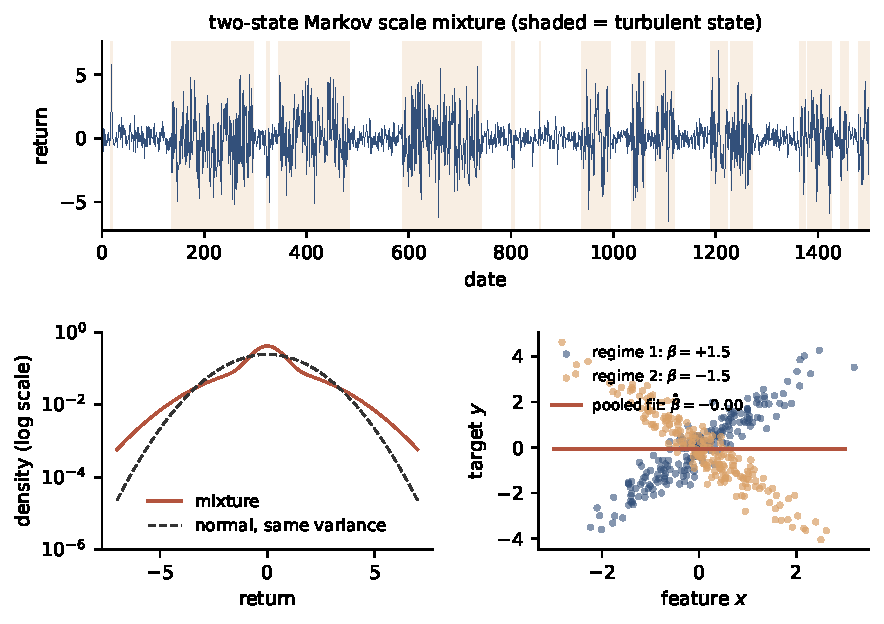
\includegraphics[width=\textwidth]{figures/regimes.pdf}
\caption{\textbf{Regimes generate the stylized facts.} Top: a return series
from a two-state Markov scale mixture ($\sigma = (0.6, 2.2)$, stay
probability $0.98$); turbulent-state periods shaded. Volatility clustering
is visible to the naked eye --- and provably absent if the same states are
shuffled i.i.d. Bottom left: the unconditional density against a Gaussian
of identical variance (log scale) --- fat tails from
Proposition~\ref{prop:kurtosis}. Bottom right: the sign-flip construction of
Section~\ref{sec:signflip} --- two regimes with slopes $\pm\beta$; the
pooled fit (red) estimates $\hat\beta \approx 0$ and is structurally blind
to a relationship that is perfectly strong within each regime.}
\label{fig:regimes}
\end{figure}

\subsection{Clustering requires persistence}\label{sec:persistence}

Fact (F1) needed only a \emph{mixture}. Fact (F2) --- clustering --- needs
more: it is a statement about \emph{dependence over time}, and an i.i.d.\
state sequence cannot produce it. If $S_t$ is drawn independently each day,
then $r_t^2$ and $r_{t+s}^2$ are independent for $s \ge 1$, so
$\Corr(r_t^2, r_{t+s}^2) = 0$: an i.i.d.\ mixture has fat tails but no
memory. Clustering is evidence that the state \emph{persists}.

The minimal persistent-state model is a Markov chain. Let $S_t$ be a
two-state chain with stay probabilities $a = \Prob(S_{t+1}{=}1 \mid S_t{=}1)$
and $b = \Prob(S_{t+1}{=}2 \mid S_t{=}2)$, and $r_t = \sigma_{S_t}\,
\varepsilon_t$ with $\varepsilon_t$ i.i.d.\ standard normal.

\begin{proposition}[Squared-return autocorrelation]\label{prop:acf}
Under the two-state Markov scale mixture, for lags $s \geq 1$,
\[
  \Corr\bigl(r_t^2,\; r_{t+s}^2\bigr)
  \;=\; c \cdot \lambda^{s},
  \qquad \lambda = a + b - 1,
\]
where $c \in (0, 1)$ is a constant depending on
$(a, b, \sigma_1, \sigma_2)$ but not on $s$. The chain's second eigenvalue
$\lambda$ --- its persistence --- is the decay rate of volatility
clustering.
\end{proposition}

\begin{proof}
Write $v_t = \sigma^2_{S_t}$, so $r_t^2 = v_t \varepsilon_t^2$ with
$\varepsilon_t^2$ i.i.d., mean $1$, independent of the state path. Then for
$s \ge 1$, $\Cov(r_t^2, r_{t+s}^2) = \Cov(v_t, v_{t+s})$ (the independent
$\varepsilon^2$ factors contribute $\E[\varepsilon^2]^2 = 1$ across distinct
times), while $\Var(r_t^2) = \E[v_t^2]\E[\varepsilon^4] - \E[v_t]^2 =
3\E[v_t^2] - \E[v_t]^2 > \Var(v_t)$; hence the correlation of $r^2$ is a
fixed positive multiple $c < 1$ of the correlation of $v$. It remains to
compute $\Corr(v_t, v_{t+s})$. The transition matrix
$A = \bigl(\begin{smallmatrix} a & 1-a \\ 1-b & b \end{smallmatrix}\bigr)$
has eigenvalues $1$ and $\lambda = a + b - 1$; its stationary distribution
is $\bar\pi = \bigl(\frac{1-b}{2-a-b}, \frac{1-a}{2-a-b}\bigr)$. For a
two-state chain, any function $f(S_t)$ --- here $v_t$, which takes two
values --- has autocorrelation exactly $\lambda^s$: decompose $f$ into its
stationary mean plus a component along the second left-eigenvector; the
$s$-step transition operator scales that component by $\lambda^s$, and
correlations are invariant to the affine part. Therefore
$\Corr(v_t, v_{t+s}) = \lambda^s$ and
$\Corr(r_t^2, r_{t+s}^2) = c\,\lambda^s$.
\end{proof}

With stay probabilities $a = b = 0.98$ (mean regime duration
$1/(1-a) = 50$ days), $\lambda = 0.96$: squared-return autocorrelations
decay by only $\sim\!4\%$ per day and remain visible for months ---
matching (F2). The top panel of Figure~\ref{fig:regimes} is this process,
and the clustering is unmistakable.

Two lessons transfer directly to the thesis model. First, \emph{persistence
is where the memory lives}: the conditional distribution of $r_t$ given the
state needs no dependence structure at all; the Markov chain carries all of
it. This division of labor --- simple emissions, dynamic state --- is
exactly the architecture of Part~II's models. Second, mean regime duration
$1/(1-a)$ gives persistence an interpretable scale, which will return in
Part~III as a \emph{persistence-biased initialization}: the learned
transition matrix is initialized sticky ($a$ near $0.9$--$0.98$), encoding
the prior belief that regimes last weeks, not hours.

\begin{origins}[Hamilton 1989 and what came before]
Mixture-of-normals descriptions of speculative prices go back to Mandelbrot
(1963) and Fama (1965) on fat tails, and to Clark (1973), whose subordinated
process --- returns as Gaussians with a randomized variance --- is
Proposition~\ref{prop:kurtosis} in continuous form. Engle's ARCH (1982) and
Bollerslev's GARCH (1986) capture clustering with an observable, recursively
defined variance. The regime-switching alternative is due to James D.
Hamilton, ``A New Approach to the Economic Analysis of Nonstationary Time
Series and the Business Cycle'' (\emph{Econometrica}, 1989): an
autoregression whose parameters switch according to an unobserved two-state
Markov chain, estimated on U.S.\ GNP growth, with the states identified
ex post as expansions and recessions --- NBER-dated recessions were
recovered by the filter without ever being shown to it. Hamilton's technical
contribution is the estimation machinery: because the state is latent, the
likelihood must integrate over all state paths, which his \emph{forward
filter} accomplishes recursively in $O(TK^2)$. That filter --- and the
distinction between filtering ($\Prob(S_t \mid \text{data up to } t)$),
which is causal, and smoothing ($\Prob(S_t \mid \text{all data})$), which
is not --- is derived in full in Chapter~7 and sits verbatim inside the
thesis model's HMM gate. The classical Hamilton model itself survives in the
package as \code{ExpertConfig(kind="classical")} $\times$
\code{PriorConfig(kind="hmm")}: constant per-regime Gaussians under a
learned Markov prior, used as a parameter-recovery test bed and an honest
classical baseline.
\end{origins}

\section{From marginal regimes to conditional regimes}\label{sec:conditional}

Everything so far concerned the \emph{marginal} distribution of returns ---
enough for risk modeling, but not yet a prediction model. The thesis takes
one further step, and it is the step that turns regime modeling into
cross-sectional alpha research:

\begin{center}
\emph{Let the map from characteristics to expected returns\\
depend on the regime.}
\end{center}

\subsection{The economics: momentum as the canonical example}

Fact (F3) is best seen through the best-documented cross-sectional signal:
momentum (buy the past year's winners, short the losers; Jegadeesh and
Titman, 1993). Its average profitability is among the most replicated
findings in finance --- and so are its \emph{crashes}. Daniel and Moskowitz
(``Momentum crashes,'' \emph{JFE}, 2016) document that momentum's worst
episodes are concentrated in a specific, identifiable state: panic markets
--- high volatility, following a market decline --- especially at the turn
into a sharp rebound. In 1932 and 2009, the losers-rebound effect was so
violent that the strategy lost most of a century's compounding in weeks. In
the language of this book: the coefficient linking the momentum
characteristic to expected return is positive in calm states and
\emph{negative} in high-volatility rebound states. Similar state-dependence
is documented for reversal strength, size, quality, and the
low-vol anomaly; regime-dependent factor performance is the working
assumption of practitioner asset allocation.

For prediction, this is qualitatively different from (F1)--(F2). A signal
whose \emph{sign flips} with the state is invisible to any model that
assumes one global mapping --- not weakened, \emph{invisible}, as the next
subsection makes exact.

\subsection{The statistics: what pooling destroys}\label{sec:signflip}

Idealize the situation. Two regimes, equally likely; within regime $k$ the
cross-section obeys a linear model with regime-dependent slope:
\[
  y_i \;=\; \beta_{S}\, x_i + \varepsilon_i,
  \qquad
  \beta_1 = +\beta,\;\; \beta_2 = -\beta,
  \qquad
  \varepsilon_i \sim \gauss(0, \sigma_\varepsilon^2),
\]
with $x_i$ standardized and independent of the regime. What does the best
\emph{global} (regime-blind) model do?

\begin{proposition}[Pooling annihilates a sign-flipping signal]
\label{prop:signflip}
Under the model above, the population regression of $y$ on $x$, pooled over
regimes, has slope
\[
  \beta_{\mathrm{pool}}
  = \frac{\Cov(y, x)}{\Var(x)}
  = \E[\beta_S]
  = \tfrac12 \beta + \tfrac12 (-\beta) = 0 ,
\]
and the pooled model's cross-sectional $R^2$ --- hence its IC --- is zero.
An oracle that knows $S$ attains
$R^2 = \beta^2 / (\beta^2 + \sigma_\varepsilon^2)$ in every regime.
Moreover, no measurable function $f(x)$ of the characteristic alone can do
better than the pooled slope: $\E[y \mid x] = \E[\beta_S]\,x = 0$ for all
$x$.
\end{proposition}

\begin{proof}
$\Cov(y, x) = \E[\beta_S x^2] + \E[\varepsilon x] = \E[\beta_S]\E[x^2]$
by independence of $S$ and $x$ and exogeneity of $\varepsilon$; the last
claim is the tower property: $\E[y \mid x] = \E[\E[y \mid x, S] \mid x] =
x\,\E[\beta_S] = 0$.
\end{proof}

The final clause is the sharp one: the failure is not linearity. \emph{Any}
model --- a gradient-boosted forest, a deep network --- that consumes only
the characteristic has zero predictive content in this world, because the
conditional mean given the characteristic alone is identically zero. The
information is real (the oracle's $R^2$ can be near $1$) but it lives
entirely in the \emph{interaction} between the characteristic and the state.
Figure~\ref{fig:regimes} (bottom right) draws the picture: two clean
regressions of slope $\pm 1.5$; one flat, useless pooled line.

This construction is deliberately extreme --- real regime-dependence is a
matter of degree, attenuation rather than annihilation (if regime
probabilities are $p \ne \tfrac12$ or slopes merely shrink, the pooled slope
is $\E[\beta_S] \ne 0$ and pooling loses part of the signal). But its
extremity is precisely what makes it \emph{useful}: it is the ideal
\textbf{planted truth} for testing a regime model. In a world generated by
Proposition~\ref{prop:signflip}, a working regime-conditional model must
achieve high IC while every regime-blind baseline must, by mathematics
rather than by luck, achieve none. The package's synthetic panel generator
implements exactly this world, and the claim ``the mixture beats the pooled
baseline \emph{here}'' is enforced as a permanent regression test --- both
directions of it (the baselines must also \emph{win} on a no-regime world,
proving they are not straw men). Chapter~14 builds the instrument; the walk-through
below shows its heart.

\begin{whatbreaks}[if regimes are real and the model is global]
Proposition~\ref{prop:signflip} is the precise content of the claim
``non-stationarity is not just drift'' from
Section~\ref{sec:hostile}. Where relationships flip with the state, a global
model does not degrade gracefully --- it averages the states and reports
noise. Worse, it does so \emph{silently}: the fit succeeds, the loss
decreases, the diagnostics look ordinary; only the out-of-sample IC hovers
at zero. If a rich global model is given extra capacity it will typically
\emph{overfit within-sample noise} before it discovers a state interaction
it has no features to express. The failure mode is invisible without a
regime-aware alternative to compare against --- one of the quieter reasons
to build the mixture even if one ultimately bets against it.
\end{whatbreaks}

\subsection{Why not just add state features?}\label{sec:whynotfeatures}

Proposition~\ref{prop:signflip} shows the model must see \emph{some} state
information. The obvious cheap fix: append a state proxy (VIX, trailing
market volatility) as a feature to a global model, and let it learn the
interaction, e.g.\ $\hat y = g(x, v)$. With enough capacity, $g$ can
represent $\beta(v)\,x$; a universal approximator handles it in principle.
Why, then, an explicit mixture? Four reasons, in increasing order of
importance to the thesis:

\begin{enumerate}[leftmargin=2em]
\item \emph{Statistical structure.} The mixture encodes the hypothesis as
  \emph{a small number of discrete states, each with a full, simple
  cross-sectional model, plus persistence in the state process}. A generic
  interaction model must discover discreteness, persistence, and the
  within-state models from scratch, spending capacity (hence variance ---
  Section~\ref{sec:hostile}) on what the mixture gets as inductive bias. In
  a domain where variance is the binding constraint, inductive bias is not a
  convenience; it is the budget.
\item \emph{Distributional honesty.} The mixture is a model of
  $p(y \mid \vx)$ with state-dependent $\sigma_k$ --- it natively expresses
  ``high-vol state $\Rightarrow$ wider predictive distribution,'' which is
  (F1)--(F2) speaking, and it is graded on it via NLL
  (Section~\ref{sec:whatisresult}). A point-prediction interaction model
  expresses none of this.
\item \emph{The state is latent.} VIX is a proxy, not the state. A mixture
  with a learned gate can \emph{infer} the state from inputs (and, in the
  HMM variant, from its own recent posterior --- carrying the persistence of
  Section~\ref{sec:persistence} into inference). Hamilton's central lesson
  applies: treat the state as unobserved and integrate over it, rather than
  hard-coding a proxy.
\item \emph{Falsifiability.} This is the decisive one for a thesis. In the
  mixture, the state is an explicit object: one can ask ``do the learned
  regimes correspond to anything real?'' and answer by correlating the
  gate's inferred posterior with \emph{held-out} state proxies it never saw
  in training (the alignment analysis of Chapter~18's practicum
  cousin, Stage~C). In a monolithic $g(x, v)$, the regime hypothesis is
  smeared across weights, and no such question can be asked. Crucially, this
  requires the gate to be \emph{unsupervised} --- the moment one trains the
  gate to predict VIX, ``the model discovered volatility regimes'' becomes
  circular. That is Decision~B of Part~III, made here, in the theory, before
  any code.
\end{enumerate}

The honest counterpoint is also worth recording: the mixture buys these
properties at the price of a harder optimization landscape (multimodality,
symmetric local optima --- Chapter~8), an identifiability problem (labels
can permute --- Chapters~7--8), and more machinery to get wrong. The
prototype of Chapter~\ref{ch:autopsy} is what ``more machinery to get
wrong'' looks like in practice. The thesis is precisely the wager that the
structure is worth its optimization cost --- and Part~V exists so that the
wager is settled by evidence rather than by enthusiasm.

\section{The model class}\label{sec:modelclass}

We can now write down the object this book builds. Everything later --- the
loss (Chapter~5), the routing variants (Chapter~6), the HMM gate
(Chapter~7), the architecture (Part~III), the evaluation (Part~V) --- is
this definition, taken seriously.

\begin{definition}[Regime-conditional mixture of experts]\label{def:nec}
For a name--date pair with features
$\vx = (\vx^{\text{seq}}, \vx^{\text{snap}})$, the model is the conditional
mixture
\[
  p(y \mid \vx)
  \;=\; \sum_{k=1}^{K} \pi_k \,\gauss\!\bigl(y;\; \mu_k(\vx),\, \sigma_k^2\bigr),
\]
with three learned ingredients:
\begin{itemize}[leftmargin=2em]
\item \textbf{Experts} $\mu_k(\cdot)$: $K$ regime-specialized prediction
  functions (small MLPs on the snapshot features; or constants, recovering
  the classical Hamilton emission), each with its own volatility
  $\sigma_k$;
\item \textbf{A gate}, producing the mixture weights from the encoded
  sequence state $\vh = \mathrm{enc}(\vx^{\text{seq}})$;
\item \textbf{A prior mechanism} $\vpi = \mathrm{prior}(\vz, \cdot)$
  turning the gate's logits $\vz(\vh)$ into weights --- \emph{pluggable}:
  a memoryless softmax $\pi_k \propto e^{z_k}$ (and its uniform / hard /
  top-$k$ / annealed variants) for thesis Variation~2, or a causal Markov
  filter $\pi_{t,k} \propto \sum_j A_{jk}\, r_{t-1,j}$ carrying yesterday's
  posterior through a learned transition matrix for Variation~3.
\end{itemize}
Training maximizes the likelihood of held-out-able data --- equivalently,
minimizes $\NLL = -\frac1n\sum \log p(y \mid \vx)$ --- with the latent state
never observed and the gate never supervised.
\end{definition}

Each clause of Definition~\ref{def:nec} answers to a section of these first
two chapters. Conditional Gaussians with per-regime $\sigma_k$: fat tails
and honest uncertainty (Proposition~\ref{prop:kurtosis},
\S\ref{sec:whatisresult}). Regime-indexed $\mu_k(\vx)$: the sign-flip
argument (Proposition~\ref{prop:signflip}). A latent, unsupervised state
inferred by a gate: \S\ref{sec:whynotfeatures}. A pluggable prior with a
Markov option: persistence (Proposition~\ref{prop:acf}) and Hamilton's
filter. Small experts on snapshot features, a small encoder for the state:
the variance budget of \S\ref{sec:hostile}. Nothing in the model is
unmotivated; that is what a design derived from theory looks like, and
Part~III will hold the implementation to it.

\begin{codewalk}[nec\_moe/data.py --- the planted world]
The synthetic generator is Proposition~\ref{prop:signflip} plus
Proposition~\ref{prop:acf} in about a page of code. Its spec exposes exactly
the theory's knobs:

\begin{lstlisting}
@dataclass(frozen=True)
class SyntheticSpec:
    n_regimes: int = 2
    regime_process: str = "iid"    # "iid" | "markov"
    transition_stay: float = 0.95  # Markov persistence  (Prop 2.2)
    vol_levels: tuple = (0.5, 2.5) # sigma_k             (Prop 2.1)
    beta_scale: float = 1.0        # +/- beta sign flip  (Prop 2.3)
    noise_std: float = 0.5         # sigma_eps
    seed: int = 0
\end{lstlisting}

Per date, one regime $S_t$ is drawn (i.i.d.\ or sticky-Markov); every name's
target is $y_{i,t} = \beta_{S_t}^\top \vx^{\text{snap}}_{i,t} +
\sigma_{S_t}\,\varepsilon_{i,t}$ with $\beta_2 = -\beta_1$ --- the sign
flip. The sequence features carry a volatility footprint of the regime, so
the state is \emph{inferable but not given}. Because the generator also
returns the true $S_t$, tests can score regime recovery directly. The two
process modes matter later: \code{"iid"} suffices for the memoryless models
of Variation~2, while \code{"markov"} plants the persistence that the HMM
gate of Variation~3 must (and, in the tests, provably does) exploit.
\end{codewalk}

\exercisehead

\begin{exercise}\label{ex:2-kurt}
(\emph{Kurtosis, quantitatively.}) (a) Show
$\kappa - 3 = 3\,\Var(V)/(\E V)^2$ where $V$ is the randomized variance of
Proposition~\ref{prop:kurtosis}. (b) For the two-state case with weights
$(p, 1{-}p)$ and volatilities $(\sigma_1, \sigma_2)$, find the weight $p$
maximizing $\kappa$ at fixed $\sigma_2/\sigma_1 = 5$, and comment: why do
\emph{rare} volatile regimes generate the fattest tails? (c) Real daily
index returns show $\kappa \approx 10$--$30$, the equal-weight two-state
model of this chapter gives $\kappa \approx 5.6$, and your answer to (b)
exceeds $20$ with the same $5\times$ volatility ratio. What do these three
numbers together suggest about how much of empirical kurtosis regime
switching can explain, and about what the regime \emph{proportions} must
look like for it to do so?
\end{exercise}

\begin{exercise}\label{ex:2-acf}
(\emph{Persistence and memory.}) (a) Complete the proof of
Proposition~\ref{prop:acf} by computing the constant $c$ explicitly for
$a = b$: show
$c = \dfrac{\Var(v)}{3\E[v^2] - (\E v)^2}$ with
$v \in \{\sigma_1^2, \sigma_2^2\}$ equally likely, and evaluate $c$ and the
lag-10 autocorrelation for $\sigma = (0.6, 2.2)$, $a = 0.98$. (b) Show that
mean regime duration is geometric with mean $1/(1-a)$. (c) An
econometrician fits a GARCH(1,1) to data generated by this model. Which
GARCH parameter will absorb $\lambda$? (No proof --- one paragraph of
reasoning.)
\end{exercise}

\begin{exercise}\label{ex:2-pool}
(\emph{Pooling, beyond the symmetric case.}) Generalize
Proposition~\ref{prop:signflip}: regimes with probabilities $(p, 1{-}p)$
and slopes $(\beta_1, \beta_2)$. (a) Find $\beta_{\mathrm{pool}}$ and the
pooled $R^2$ as functions of $(p, \beta_1, \beta_2, \sigma_\varepsilon)$.
(b) Show the pooled model's \emph{residual variance} exceeds the oracle's by
$\Var(\beta_S)\,\E[x^2]$ --- regime dispersion in slopes reappears as
irreducible-looking noise. (c) Connect (b) to
Proposition~\ref{prop:kurtosis}: in what precise sense is ``variance of the
slope'' the cross-sectional analogue of ``variance of the variance''?
\end{exercise}

\begin{exercise}\label{ex:2-modes}
(\emph{When is a mixture visibly a mixture?}) For the equal-weight,
equal-variance two-component mixture
$\tfrac12\gauss(\mu_1, \sigma^2) + \tfrac12\gauss(\mu_2, \sigma^2)$, show
the density is bimodal if and only if $|\mu_1 - \mu_2| > 2\sigma$.
(Reduce to $f(x) \propto \cosh(\delta x)e^{-x^2/2}$ form and study its
critical points.) Conclude: regime structure can be strong yet invisible in
the marginal density --- which is why Chapter~14's planted-truth tests grade
models on \emph{recovery of the latent state}, never on eyeballing
histograms.
\end{exercise}

\begin{exercise}\label{ex:2-hands}
(\emph{Hands-on: verify the theory against the generator.}) Using
\code{SyntheticRegimePanel} with the defaults of the code walkthrough:
(a) simulate $50{,}000$ dates of the \code{"markov"} process
(\code{transition\_stay}=0.98) and verify Proposition~\ref{prop:kurtosis}'s
kurtosis and Proposition~\ref{prop:acf}'s geometric ACF decay numerically
(log-ACF should be linear in lag with slope $\log\lambda$);
(b) regress $y$ on the snapshot features pooled versus within-regime (the
generator exposes true regimes) and reproduce
Proposition~\ref{prop:signflip}'s zero-versus-oracle contrast;
(c) switch to \code{regime\_process="iid"} and confirm the ACF flattens
while the kurtosis survives --- the cleanest possible demonstration that
tails come from \emph{mixing} but memory comes from \emph{persistence}.
\end{exercise}
